\documentclass[]{article}
\usepackage{lmodern}
\usepackage{amssymb,amsmath}
\usepackage{ifxetex,ifluatex}
\usepackage{fixltx2e} % provides \textsubscript
\ifnum 0\ifxetex 1\fi\ifluatex 1\fi=0 % if pdftex
  \usepackage[T1]{fontenc}
  \usepackage[utf8]{inputenc}
\else % if luatex or xelatex
  \ifxetex
    \usepackage{mathspec}
    \usepackage{xltxtra,xunicode}
  \else
    \usepackage{fontspec}
  \fi
  \defaultfontfeatures{Mapping=tex-text,Scale=MatchLowercase}
  \newcommand{\euro}{€}
\fi
% use upquote if available, for straight quotes in verbatim environments
\IfFileExists{upquote.sty}{\usepackage{upquote}}{}
% use microtype if available
\IfFileExists{microtype.sty}{%
\usepackage{microtype}
\UseMicrotypeSet[protrusion]{basicmath} % disable protrusion for tt fonts
}{}
\usepackage[margin=1in]{geometry}
\usepackage{color}
\usepackage{fancyvrb}
\newcommand{\VerbBar}{|}
\newcommand{\VERB}{\Verb[commandchars=\\\{\}]}
\DefineVerbatimEnvironment{Highlighting}{Verbatim}{commandchars=\\\{\}}
% Add ',fontsize=\small' for more characters per line
\usepackage{framed}
\definecolor{shadecolor}{RGB}{248,248,248}
\newenvironment{Shaded}{\begin{snugshade}}{\end{snugshade}}
\newcommand{\KeywordTok}[1]{\textcolor[rgb]{0.13,0.29,0.53}{\textbf{{#1}}}}
\newcommand{\DataTypeTok}[1]{\textcolor[rgb]{0.13,0.29,0.53}{{#1}}}
\newcommand{\DecValTok}[1]{\textcolor[rgb]{0.00,0.00,0.81}{{#1}}}
\newcommand{\BaseNTok}[1]{\textcolor[rgb]{0.00,0.00,0.81}{{#1}}}
\newcommand{\FloatTok}[1]{\textcolor[rgb]{0.00,0.00,0.81}{{#1}}}
\newcommand{\CharTok}[1]{\textcolor[rgb]{0.31,0.60,0.02}{{#1}}}
\newcommand{\StringTok}[1]{\textcolor[rgb]{0.31,0.60,0.02}{{#1}}}
\newcommand{\CommentTok}[1]{\textcolor[rgb]{0.56,0.35,0.01}{\textit{{#1}}}}
\newcommand{\OtherTok}[1]{\textcolor[rgb]{0.56,0.35,0.01}{{#1}}}
\newcommand{\AlertTok}[1]{\textcolor[rgb]{0.94,0.16,0.16}{{#1}}}
\newcommand{\FunctionTok}[1]{\textcolor[rgb]{0.00,0.00,0.00}{{#1}}}
\newcommand{\RegionMarkerTok}[1]{{#1}}
\newcommand{\ErrorTok}[1]{\textbf{{#1}}}
\newcommand{\NormalTok}[1]{{#1}}
\usepackage{graphicx}
\makeatletter
\def\maxwidth{\ifdim\Gin@nat@width>\linewidth\linewidth\else\Gin@nat@width\fi}
\def\maxheight{\ifdim\Gin@nat@height>\textheight\textheight\else\Gin@nat@height\fi}
\makeatother
% Scale images if necessary, so that they will not overflow the page
% margins by default, and it is still possible to overwrite the defaults
% using explicit options in \includegraphics[width, height, ...]{}
\setkeys{Gin}{width=\maxwidth,height=\maxheight,keepaspectratio}
\ifxetex
  \usepackage[setpagesize=false, % page size defined by xetex
              unicode=false, % unicode breaks when used with xetex
              xetex]{hyperref}
\else
  \usepackage[unicode=true]{hyperref}
\fi
\hypersetup{breaklinks=true,
            bookmarks=true,
            pdfauthor={Charles Brown},
            pdftitle={Lab 3A: Foundataions for inference - Sampling Disributions},
            colorlinks=true,
            citecolor=blue,
            urlcolor=blue,
            linkcolor=magenta,
            pdfborder={0 0 0}}
\urlstyle{same}  % don't use monospace font for urls
\setlength{\parindent}{0pt}
\setlength{\parskip}{6pt plus 2pt minus 1pt}
\setlength{\emergencystretch}{3em}  % prevent overfull lines
\setcounter{secnumdepth}{5}

%%% Use protect on footnotes to avoid problems with footnotes in titles
\let\rmarkdownfootnote\footnote%
\def\footnote{\protect\rmarkdownfootnote}

%%% Change title format to be more compact
\usepackage{titling}

% Create subtitle command for use in maketitle
\newcommand{\subtitle}[1]{
  \posttitle{
    \begin{center}\large#1\end{center}
    }
}

\setlength{\droptitle}{-2em}
  \title{Lab 3A: Foundataions for inference - Sampling Disributions}
  \pretitle{\vspace{\droptitle}\centering\huge}
  \posttitle{\par}
  \author{Charles Brown}
  \preauthor{\centering\large\emph}
  \postauthor{\par}
  \predate{\centering\large\emph}
  \postdate{\par}
  \date{Sunday, March 29, 2015}



\begin{document}

\maketitle


{
\hypersetup{linkcolor=black}
\setcounter{tocdepth}{2}
\tableofcontents
}
\subsubsection{Load Data}\label{load-data}

\begin{Shaded}
\begin{Highlighting}[]
\KeywordTok{load}\NormalTok{(}\DataTypeTok{file =} \KeywordTok{url}\NormalTok{(}\StringTok{"http://www.openintro.org/stat/data/ames.RData"}\NormalTok{))}
\end{Highlighting}
\end{Shaded}

\begin{center}\rule{0.5\linewidth}{\linethickness}\end{center}

\subsubsection{Exploratory Stats}\label{exploratory-stats}

\begin{Shaded}
\begin{Highlighting}[]
\KeywordTok{sort}\NormalTok{(}\KeywordTok{names}\NormalTok{(ames))}
\end{Highlighting}
\end{Shaded}

\begin{verbatim}
##  [1] "Alley"           "Bedroom.AbvGr"   "Bldg.Type"      
##  [4] "Bsmt.Cond"       "Bsmt.Exposure"   "Bsmt.Full.Bath" 
##  [7] "Bsmt.Half.Bath"  "Bsmt.Qual"       "Bsmt.Unf.SF"    
## [10] "BsmtFin.SF.1"    "BsmtFin.SF.2"    "BsmtFin.Type.1" 
## [13] "BsmtFin.Type.2"  "Central.Air"     "Condition.1"    
## [16] "Condition.2"     "Electrical"      "Enclosed.Porch" 
## [19] "Exter.Cond"      "Exter.Qual"      "Exterior.1st"   
## [22] "Exterior.2nd"    "Fence"           "Fireplace.Qu"   
## [25] "Fireplaces"      "Foundation"      "Full.Bath"      
## [28] "Functional"      "Garage.Area"     "Garage.Cars"    
## [31] "Garage.Cond"     "Garage.Finish"   "Garage.Qual"    
## [34] "Garage.Type"     "Garage.Yr.Blt"   "Gr.Liv.Area"    
## [37] "Half.Bath"       "Heating"         "Heating.QC"     
## [40] "House.Style"     "Kitchen.AbvGr"   "Kitchen.Qual"   
## [43] "Land.Contour"    "Land.Slope"      "Lot.Area"       
## [46] "Lot.Config"      "Lot.Frontage"    "Lot.Shape"      
## [49] "Low.Qual.Fin.SF" "Mas.Vnr.Area"    "Mas.Vnr.Type"   
## [52] "Misc.Feature"    "Misc.Val"        "Mo.Sold"        
## [55] "MS.SubClass"     "MS.Zoning"       "Neighborhood"   
## [58] "Open.Porch.SF"   "Order"           "Overall.Cond"   
## [61] "Overall.Qual"    "Paved.Drive"     "PID"            
## [64] "Pool.Area"       "Pool.QC"         "Roof.Matl"      
## [67] "Roof.Style"      "Sale.Condition"  "Sale.Type"      
## [70] "SalePrice"       "Screen.Porch"    "Street"         
## [73] "Total.Bsmt.SF"   "TotRms.AbvGrd"   "Utilities"      
## [76] "Wood.Deck.SF"    "X1st.Flr.SF"     "X2nd.Flr.SF"    
## [79] "X3Ssn.Porch"     "Year.Built"      "Year.Remod.Add" 
## [82] "Yr.Sold"
\end{verbatim}

\begin{Shaded}
\begin{Highlighting}[]
\CommentTok{#}
\NormalTok{area <-}\StringTok{ }\NormalTok{ames$Gr.Liv.Area}
\NormalTok{(xsum <-}\KeywordTok{summary}\NormalTok{(area))}
\end{Highlighting}
\end{Shaded}

\begin{verbatim}
##    Min. 1st Qu.  Median    Mean 3rd Qu.    Max. 
##     334    1126    1442    1500    1743    5642
\end{verbatim}

\begin{Shaded}
\begin{Highlighting}[]
\KeywordTok{hist}\NormalTok{(}\DataTypeTok{x =} \NormalTok{area, }\DataTypeTok{xlab =} \StringTok{"Area in Sq. Feet"}\NormalTok{, }\DataTypeTok{breaks =} \DecValTok{100}\NormalTok{)}
\KeywordTok{text}\NormalTok{(}\DecValTok{4000}\NormalTok{, }\DecValTok{120}\NormalTok{, }\KeywordTok{paste}\NormalTok{(}\StringTok{"Mean ="}\NormalTok{, }\KeywordTok{round}\NormalTok{(}\KeywordTok{mean}\NormalTok{(area), }\DecValTok{1}\NormalTok{), }\StringTok{"}\CharTok{\textbackslash{}n}\StringTok{ Median ="}\NormalTok{, }
         \KeywordTok{round}\NormalTok{(}\KeywordTok{median}\NormalTok{(area), }\DecValTok{1}\NormalTok{), }\StringTok{"}\CharTok{\textbackslash{}n}\StringTok{ Std.Dev ="}\NormalTok{, }\KeywordTok{round}\NormalTok{(}\KeywordTok{sd}\NormalTok{(area), }\DecValTok{1}\NormalTok{)))}
\end{Highlighting}
\end{Shaded}

\begin{figure}[htbp]
\centering
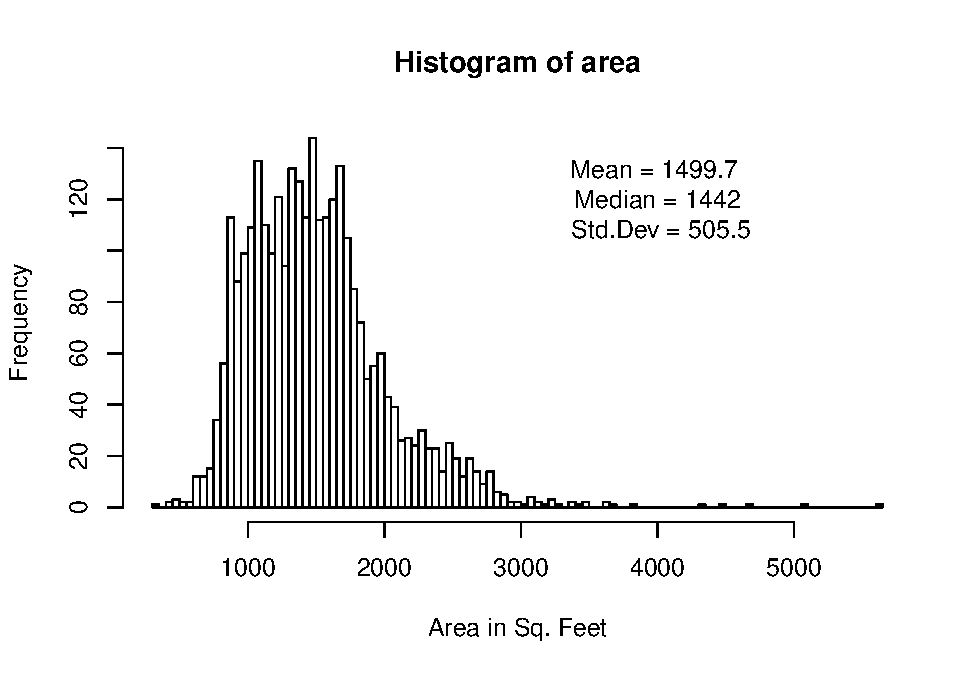
\includegraphics{Lab3A_files/figure-latex/ExploreData-1.pdf}
\caption{}
\end{figure}

\paragraph{Question 1: Which of the following is
false?}\label{question-1-which-of-the-following-is-false}

\begin{enumerate}
\def\labelenumi{\Alph{enumi})}
\itemsep1pt\parskip0pt\parsep0pt
\item
  The distribution of areas of houses in Ames is unimodal and
  right-skewed.
\item
  \textbf{50\% of houses in Ames are smaller than 1,500 square feet.}
\item
  The middle 50\% of the houses range between approximately 1,130 square
  feet and 1,740 square feet.
\item
  The IQR is approximately 610 square feet.
\item
  The smallest house is 334 square feet and the largest is 5,642 square
  feet.
\end{enumerate}

\begin{itemize}
\itemsep1pt\parskip0pt\parsep0pt
\item
  Half of the houses in Ames are less than the median of 1442 square
  feet.
\end{itemize}

\textbf{Question 1 Answer: B)}

\begin{center}\rule{0.5\linewidth}{\linethickness}\end{center}

\subsubsection{The Unknown Sampling
Distribution.}\label{the-unknown-sampling-distribution.}

\begin{Shaded}
\begin{Highlighting}[]
\NormalTok{samp0 <-}\KeywordTok{sample}\NormalTok{(area,}\DecValTok{50}\NormalTok{)}
\NormalTok{samp1 <-}\KeywordTok{sample}\NormalTok{(area,}\DecValTok{50}\NormalTok{)}
\CommentTok{#}
\KeywordTok{mean}\NormalTok{(samp1)}
\end{Highlighting}
\end{Shaded}

\begin{verbatim}
## [1] 1519.24
\end{verbatim}

\begin{Shaded}
\begin{Highlighting}[]
\KeywordTok{summary}\NormalTok{(samp1)}
\end{Highlighting}
\end{Shaded}

\begin{verbatim}
##    Min. 1st Qu.  Median    Mean 3rd Qu.    Max. 
##     672    1082    1437    1519    1847    2798
\end{verbatim}

\begin{Shaded}
\begin{Highlighting}[]
\CommentTok{#}
\NormalTok{samp_50 <-}\KeywordTok{sample}\NormalTok{(area,}\DecValTok{50}\NormalTok{)}
\NormalTok{samp_100 <-}\KeywordTok{sample}\NormalTok{(area,}\DecValTok{100}\NormalTok{)}
\NormalTok{samp_1000 <-}\KeywordTok{sample}\NormalTok{(area, }\DecValTok{1000}\NormalTok{)}
\end{Highlighting}
\end{Shaded}

\paragraph{Question 2: Suppose we took two more samples, one of size 100
and one of size 1000. Which would you think would provide a more
accurate estimate of the population
mean?}\label{question-2-suppose-we-took-two-more-samples-one-of-size-100-and-one-of-size-1000.-which-would-you-think-would-provide-a-more-accurate-estimate-of-the-population-mean}

\begin{enumerate}
\def\labelenumi{\Alph{enumi})}
\itemsep1pt\parskip0pt\parsep0pt
\item
  Sample size of 50
\item
  Sample size of 100
\item
  \textbf{Sample size of 1000}
\end{enumerate}

\begin{itemize}
\itemsep1pt\parskip0pt\parsep0pt
\item
  Mean of Entire Population of : 1499.6904437.
\item
  Mean of Sample size 50: 1421.76.
\item
  Mean of Sample size 100: 1480.64.
\item
  Mean of sample size 1000: 1518.348.
\end{itemize}

\textbf{Question 2 Answer: The larger the sample size, the better the
estimate of the mean.}

The distribution of sample means, called the sampling distribution, can
help us understand this variability. In this lab, because we have access
to the population, we can build up the sampling distribution for the
sample mean by repeating the above steps many times. Here we will
generate 5000 samples and compute the sample mean of each.

\begin{Shaded}
\begin{Highlighting}[]
\NormalTok{sample_means50 <-}\StringTok{ }\KeywordTok{rep}\NormalTok{(}\OtherTok{NA}\NormalTok{, }\DecValTok{5000}\NormalTok{)}

\NormalTok{for(i in }\DecValTok{1}\NormalTok{:}\DecValTok{5000}\NormalTok{)\{}
   \NormalTok{samp <-}\StringTok{ }\KeywordTok{sample}\NormalTok{(area, }\DecValTok{50}\NormalTok{)}
   \NormalTok{sample_means50[i] <-}\StringTok{ }\KeywordTok{mean}\NormalTok{(samp)}
   \NormalTok{\}}

\NormalTok{(xsum <-}\KeywordTok{summary}\NormalTok{(sample_means50))}
\end{Highlighting}
\end{Shaded}

\begin{verbatim}
##    Min. 1st Qu.  Median    Mean 3rd Qu.    Max. 
##    1265    1451    1499    1501    1548    1771
\end{verbatim}

\begin{Shaded}
\begin{Highlighting}[]
\KeywordTok{hist}\NormalTok{(sample_means50, }\DataTypeTok{breaks =} \DecValTok{50}\NormalTok{)}
\KeywordTok{text}\NormalTok{(}\DecValTok{1725}\NormalTok{, }\DecValTok{250}\NormalTok{, }\KeywordTok{paste}\NormalTok{(}\StringTok{"Mean ="}\NormalTok{, }\KeywordTok{round}\NormalTok{(}\KeywordTok{mean}\NormalTok{(sample_means50), }\DecValTok{1}\NormalTok{), }\StringTok{"}\CharTok{\textbackslash{}n}\StringTok{ Median ="}\NormalTok{, }
         \KeywordTok{round}\NormalTok{(}\KeywordTok{median}\NormalTok{(sample_means50), }\DecValTok{1}\NormalTok{), }\StringTok{"}\CharTok{\textbackslash{}n}\StringTok{ Std.Dev ="}\NormalTok{, }\KeywordTok{round}\NormalTok{(}\KeywordTok{sd}\NormalTok{(sample_means50), }\DecValTok{1}\NormalTok{)))}
\end{Highlighting}
\end{Shaded}

\begin{figure}[htbp]
\centering
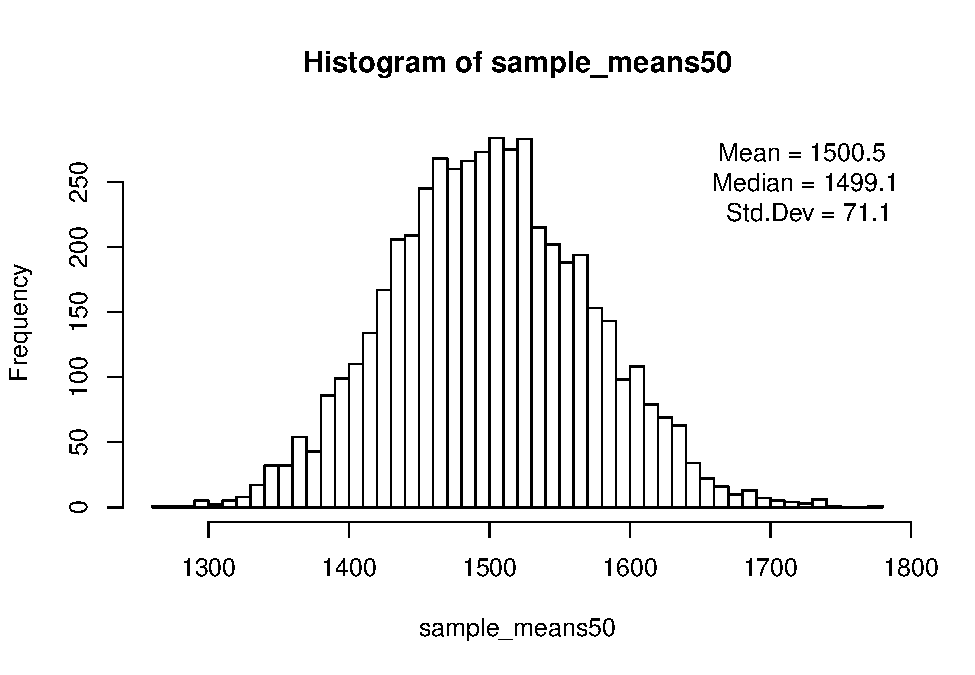
\includegraphics{Lab3A_files/figure-latex/SamplingDistPlot-1.pdf}
\caption{}
\end{figure}

\begin{Shaded}
\begin{Highlighting}[]
\KeywordTok{summary}\NormalTok{(sample_means50)}
\end{Highlighting}
\end{Shaded}

\begin{verbatim}
##    Min. 1st Qu.  Median    Mean 3rd Qu.    Max. 
##    1265    1451    1499    1501    1548    1771
\end{verbatim}

\paragraph{Exercise: Describe the sampling distribution (the
distribution of the sample means that you just created), and be sure to
specifically note its
center.}\label{exercise-describe-the-sampling-distribution-the-distribution-of-the-sample-means-that-you-just-created-and-be-sure-to-specifically-note-its-center.}

\textbf{Excercise Answer: The sampling distribution looks a like a
normal distribution with a mean of 1500.506272.}

\paragraph{Exercise: To make sure you understand what you've done in
this loop, try running a smaller version. Initialize a vector of 100 NAs
called sample\_means\_small. Run a loop that takes a sample of size 50
from area and stores the sample mean in sample\_means\_small. Print the
output to your screen (type sample\_means\_small into the console and
press
enter).}\label{exercise-to-make-sure-you-understand-what-youve-done-in-this-loop-try-running-a-smaller-version.-initialize-a-vector-of-100-nas-called-sampleux5fmeansux5fsmall.-run-a-loop-that-takes-a-sample-of-size-50-from-area-and-stores-the-sample-mean-in-sampleux5fmeansux5fsmall.-print-the-output-to-your-screen-type-sampleux5fmeansux5fsmall-into-the-console-and-press-enter.}

\begin{Shaded}
\begin{Highlighting}[]
\NormalTok{sample_means_small <-}\KeywordTok{rep}\NormalTok{(}\OtherTok{NA}\NormalTok{, }\DecValTok{100}\NormalTok{)}

\NormalTok{for (i in }\DecValTok{1}\NormalTok{:}\StringTok{ }\DecValTok{100}\NormalTok{)}
\NormalTok{\{}
     \NormalTok{samp <-}\KeywordTok{sample}\NormalTok{(area,}\DecValTok{50}\NormalTok{)}
     \NormalTok{sample_means_small[i] <-}\KeywordTok{mean}\NormalTok{(samp)}
    
\NormalTok{\}}

\NormalTok{sample_means_small}
\end{Highlighting}
\end{Shaded}

\begin{verbatim}
##   [1] 1440.52 1456.38 1546.40 1453.22 1440.46 1495.98 1469.60 1407.00
##   [9] 1532.84 1558.88 1552.46 1614.68 1468.86 1572.72 1588.06 1349.74
##  [17] 1550.36 1483.44 1451.48 1458.22 1549.62 1670.06 1631.80 1438.94
##  [25] 1588.66 1522.04 1508.46 1509.82 1496.66 1539.38 1514.88 1437.16
##  [33] 1377.64 1456.62 1424.04 1525.96 1508.68 1578.52 1446.42 1425.92
##  [41] 1470.88 1480.84 1508.82 1511.80 1494.22 1466.74 1410.76 1463.52
##  [49] 1441.52 1555.68 1487.50 1422.34 1636.46 1458.50 1479.40 1376.98
##  [57] 1477.62 1458.36 1556.12 1470.72 1553.48 1612.04 1422.36 1572.46
##  [65] 1527.26 1478.82 1492.30 1391.20 1503.06 1629.36 1468.34 1618.38
##  [73] 1437.18 1546.74 1427.26 1346.76 1428.58 1471.82 1532.70 1675.44
##  [81] 1553.94 1533.92 1469.98 1420.28 1441.96 1368.98 1445.30 1358.36
##  [89] 1570.08 1539.12 1541.44 1432.80 1611.60 1467.78 1559.06 1600.00
##  [97] 1385.70 1620.50 1418.54 1482.94
\end{verbatim}

\begin{Shaded}
\begin{Highlighting}[]
\KeywordTok{hist}\NormalTok{(sample_means_small, }\DataTypeTok{breaks =} \DecValTok{25}\NormalTok{)}
\KeywordTok{text}\NormalTok{(}\DecValTok{1650}\NormalTok{, }\DecValTok{7}\NormalTok{, }\KeywordTok{paste}\NormalTok{(}\StringTok{"Mean ="}\NormalTok{, }\KeywordTok{round}\NormalTok{(}\KeywordTok{mean}\NormalTok{(sample_means_small), }\DecValTok{1}\NormalTok{), }\StringTok{"}\CharTok{\textbackslash{}n}\StringTok{ Median ="}\NormalTok{, }
         \KeywordTok{round}\NormalTok{(}\KeywordTok{median}\NormalTok{(sample_means_small), }\DecValTok{1}\NormalTok{), }\StringTok{"}\CharTok{\textbackslash{}n}\StringTok{ Std.Dev ="}\NormalTok{, }\KeywordTok{round}\NormalTok{(}\KeywordTok{sd}\NormalTok{(sample_means_small), }\DecValTok{1}\NormalTok{)))}
\end{Highlighting}
\end{Shaded}

\begin{figure}[htbp]
\centering
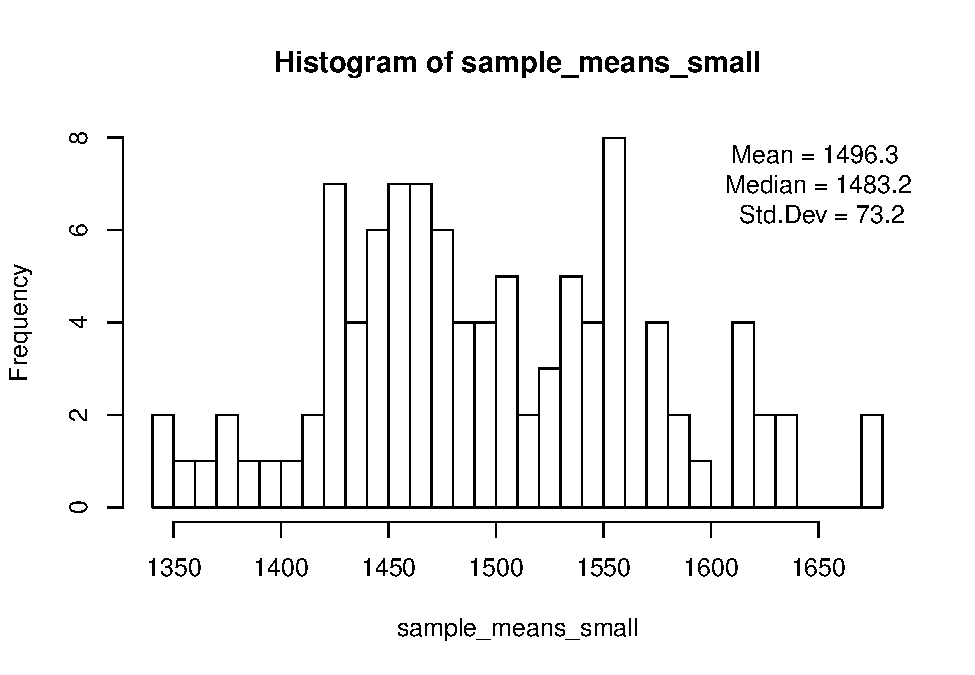
\includegraphics{Lab3A_files/figure-latex/forlooptest-1.pdf}
\caption{}
\end{figure}

\paragraph{Question 3: How many elements are there in this object called
sample\_means\_small?}\label{question-3-how-many-elements-are-there-in-this-object-called-sampleux5fmeansux5fsmall}

\begin{enumerate}
\def\labelenumi{\Alph{enumi})}
\itemsep1pt\parskip0pt\parsep0pt
\item
  0
\item
  30
\item
  50
\item
  \textbf{100}
\item
  5,000
\end{enumerate}

\textbf{Question 3 Answer: \texttt{sample\_means\_small contains} 100
elements.}

\paragraph{Question 4: Which of the following is true about the elements
in the sampling distributions you
created?}\label{question-4-which-of-the-following-is-true-about-the-elements-in-the-sampling-distributions-you-created}

\begin{enumerate}
\def\labelenumi{\Alph{enumi})}
\itemsep1pt\parskip0pt\parsep0pt
\item
  \textbf{Each element represents a mean square footage from a simple
  random sample of 50 houses.}
\item
  Each element represents the square footage of a house.
\item
  Each element represents the true population mean of square footage of
  houses.
\end{enumerate}

\textbf{Question 4 Answer: Each element of this sampling distribution
vector is a mean of a random sample (size 50) from the population.}

\begin{center}\rule{0.5\linewidth}{\linethickness}\end{center}

\subsubsection{Sample size and the sampling
distribution}\label{sample-size-and-the-sampling-distribution}

To get a sense of the effect that sample size has on our sampling
distribution, let's build up two more sampling distributions: one based
on a sample size of 10 and another based on a sample size of 100.

\begin{Shaded}
\begin{Highlighting}[]
\NormalTok{sample_means10 <-}\StringTok{ }\KeywordTok{rep}\NormalTok{(}\OtherTok{NA}\NormalTok{, }\DecValTok{5000}\NormalTok{)}
\NormalTok{sample_means100 <-}\StringTok{ }\KeywordTok{rep}\NormalTok{(}\OtherTok{NA}\NormalTok{, }\DecValTok{5000}\NormalTok{)}

\NormalTok{for(i in }\DecValTok{1}\NormalTok{:}\DecValTok{5000}\NormalTok{)\{}
  \NormalTok{samp <-}\StringTok{ }\KeywordTok{sample}\NormalTok{(area, }\DecValTok{10}\NormalTok{)}
  \NormalTok{sample_means10[i] <-}\StringTok{ }\KeywordTok{mean}\NormalTok{(samp)}
  \NormalTok{samp <-}\StringTok{ }\KeywordTok{sample}\NormalTok{(area, }\DecValTok{100}\NormalTok{)}
  \NormalTok{sample_means100[i] <-}\StringTok{ }\KeywordTok{mean}\NormalTok{(samp)}
\NormalTok{\}}
\end{Highlighting}
\end{Shaded}

To see the effect that different sample sizes have on the sampling
distribution, plot the three distributions on top of one another.

\begin{Shaded}
\begin{Highlighting}[]
\KeywordTok{par}\NormalTok{(}\DataTypeTok{mfrow =} \KeywordTok{c}\NormalTok{(}\DecValTok{3}\NormalTok{, }\DecValTok{1}\NormalTok{))}
\NormalTok{xlimits =}\StringTok{ }\KeywordTok{range}\NormalTok{(sample_means10)}
\KeywordTok{hist}\NormalTok{(sample_means10, }\DataTypeTok{breaks =} \DecValTok{20}\NormalTok{, }\DataTypeTok{xlim =} \NormalTok{xlimits)}
\KeywordTok{text}\NormalTok{(}\DecValTok{1850}\NormalTok{, }\DecValTok{500}\NormalTok{, }\KeywordTok{paste}\NormalTok{(}\StringTok{"Std.Dev ="}\NormalTok{, }\KeywordTok{round}\NormalTok{(}\KeywordTok{sd}\NormalTok{(sample_means10), }\DecValTok{1}\NormalTok{)))}
\KeywordTok{hist}\NormalTok{(sample_means50, }\DataTypeTok{breaks =} \DecValTok{20}\NormalTok{, }\DataTypeTok{xlim =} \NormalTok{xlimits)}
\KeywordTok{text}\NormalTok{(}\DecValTok{1850}\NormalTok{, }\DecValTok{500}\NormalTok{, }\KeywordTok{paste}\NormalTok{(}\StringTok{"Std.Dev ="}\NormalTok{, }\KeywordTok{round}\NormalTok{(}\KeywordTok{sd}\NormalTok{(sample_means50), }\DecValTok{1}\NormalTok{)))}
\KeywordTok{hist}\NormalTok{(sample_means100, }\DataTypeTok{breaks =} \DecValTok{20}\NormalTok{, }\DataTypeTok{xlim =} \NormalTok{xlimits)}
\KeywordTok{text}\NormalTok{(}\DecValTok{1850}\NormalTok{, }\DecValTok{500}\NormalTok{, }\KeywordTok{paste}\NormalTok{(}\StringTok{"Std.Dev ="}\NormalTok{, }\KeywordTok{round}\NormalTok{(}\KeywordTok{sd}\NormalTok{(sample_means100), }\DecValTok{1}\NormalTok{)))}
\end{Highlighting}
\end{Shaded}

\begin{figure}[htbp]
\centering
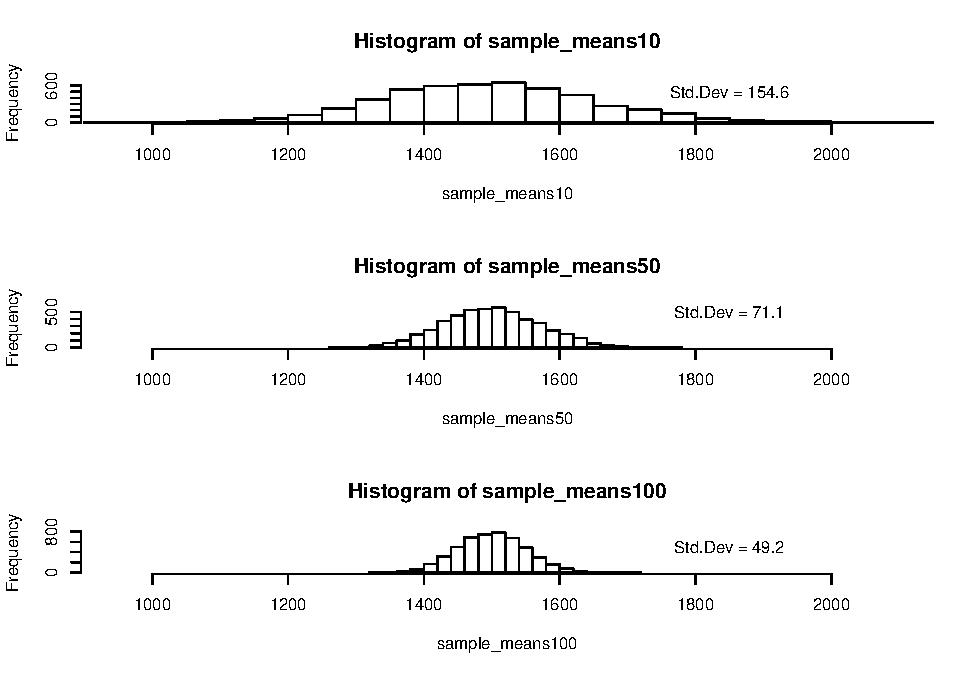
\includegraphics{Lab3A_files/figure-latex/PloSampleSizeText-1.pdf}
\caption{}
\end{figure}

\paragraph{Question 5: It makes intuitive sense that as the sample size
increases, the center of the sampling distribution becomes a more
reliable estimate for the true population mean. Also as the sample size
increases, the variability of the sampling distribution
\_\_\_\_\_\_\_\_.}\label{question-5-it-makes-intuitive-sense-that-as-the-sample-size-increases-the-center-of-the-sampling-distribution-becomes-a-more-reliable-estimate-for-the-true-population-mean.-also-as-the-sample-size-increases-the-variability-of-the-sampling-distribution-ux5fux5fux5fux5fux5fux5fux5fux5f.}

\begin{enumerate}
\def\labelenumi{\Alph{enumi})}
\itemsep1pt\parskip0pt\parsep0pt
\item
  \textbf{decreases}
\item
  increases
\item
  stays the same
\end{enumerate}

\textbf{Answer Question 5: The panel plot shows that the variability
decreases as the sample size increases.}

\begin{center}\rule{0.5\linewidth}{\linethickness}\end{center}

\subsubsection{Now you'll try to estimate the mean home
price.}\label{now-youll-try-to-estimate-the-mean-home-price.}

\paragraph{Exercise: Take a random sample of size 50 from price. Using
this sample, what is your best point estimate of the population
mean?}\label{exercise-take-a-random-sample-of-size-50-from-price.-using-this-sample-what-is-your-best-point-estimate-of-the-population-mean}

\begin{Shaded}
\begin{Highlighting}[]
\NormalTok{price <-}\StringTok{ }\NormalTok{ames$SalePrice}
\NormalTok{samp <-}\KeywordTok{sample}\NormalTok{(price,}\DecValTok{50}\NormalTok{)}
\NormalTok{(xsum <-}\KeywordTok{summary}\NormalTok{(samp))}
\end{Highlighting}
\end{Shaded}

\begin{verbatim}
##    Min. 1st Qu.  Median    Mean 3rd Qu.    Max. 
##   78000  136600  165800  188200  229600  378500
\end{verbatim}

\begin{Shaded}
\begin{Highlighting}[]
\KeywordTok{hist}\NormalTok{(samp, }\DataTypeTok{xlab =} \StringTok{"Price"}\NormalTok{, }\DataTypeTok{breaks =} \DecValTok{50}\NormalTok{)}
\end{Highlighting}
\end{Shaded}

\begin{figure}[htbp]
\centering
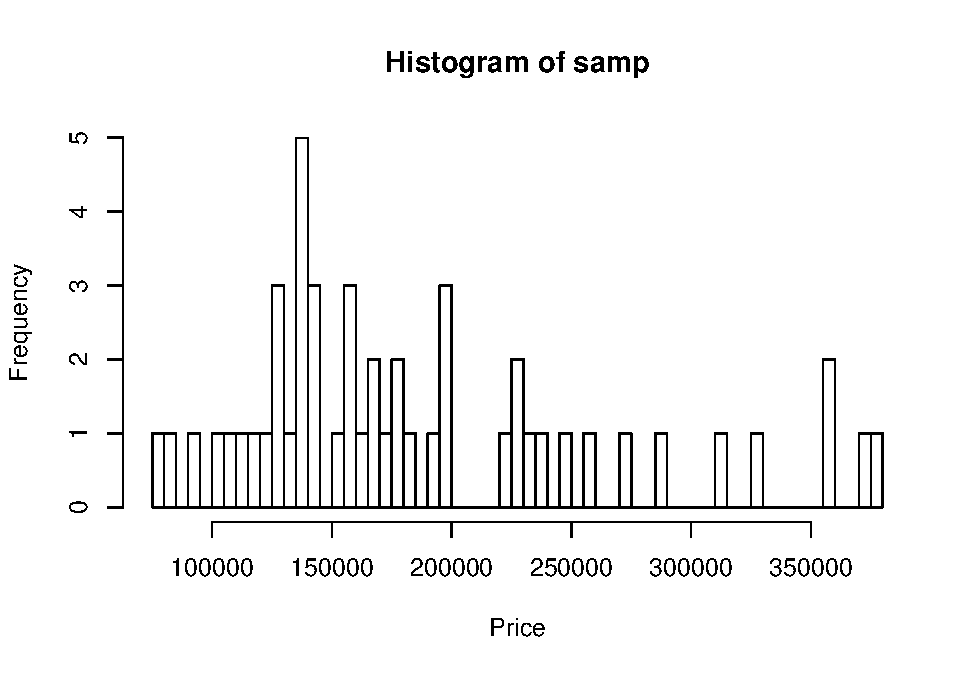
\includegraphics{Lab3A_files/figure-latex/RandomSamp50Price-1.pdf}
\caption{}
\end{figure}

\textbf{Exercise Answer: The point estimate of the mean is 188.2K.}

\paragraph{Exercise: Since you have access to the population, simulate
the sampling distribution for x¯price by taking 5000 samples from the
population of size 50 and computing 5000 sample means. Store these means
in a vector called sample\_means50. Plot the data, then describe the
shape of this sampling distribution. Based on this sampling
distribution, what would you guess the mean home price of the population
to
be?}\label{exercise-since-you-have-access-to-the-population-simulate-the-sampling-distribution-for-xprice-by-taking-5000-samples-from-the-population-of-size-50-and-computing-5000-sample-means.-store-these-means-in-a-vector-called-sampleux5fmeans50.-plot-the-data-then-describe-the-shape-of-this-sampling-distribution.-based-on-this-sampling-distribution-what-would-you-guess-the-mean-home-price-of-the-population-to-be}

\begin{Shaded}
\begin{Highlighting}[]
\NormalTok{sample_means50 <-}\KeywordTok{rep}\NormalTok{(}\OtherTok{NA}\NormalTok{,}\DecValTok{5000}\NormalTok{)}

\NormalTok{for (i in }\DecValTok{1}\NormalTok{:}\DecValTok{5000}\NormalTok{)}
\NormalTok{\{}
     \NormalTok{samp <-}\KeywordTok{sample}\NormalTok{(price, }\DecValTok{50}\NormalTok{)}
     \NormalTok{sample_means50[i] <-}\KeywordTok{mean}\NormalTok{(samp)}
\NormalTok{\}}

\KeywordTok{hist}\NormalTok{(sample_means50, }\DataTypeTok{breaks =} \DecValTok{50}\NormalTok{)}
\end{Highlighting}
\end{Shaded}

\begin{figure}[htbp]
\centering
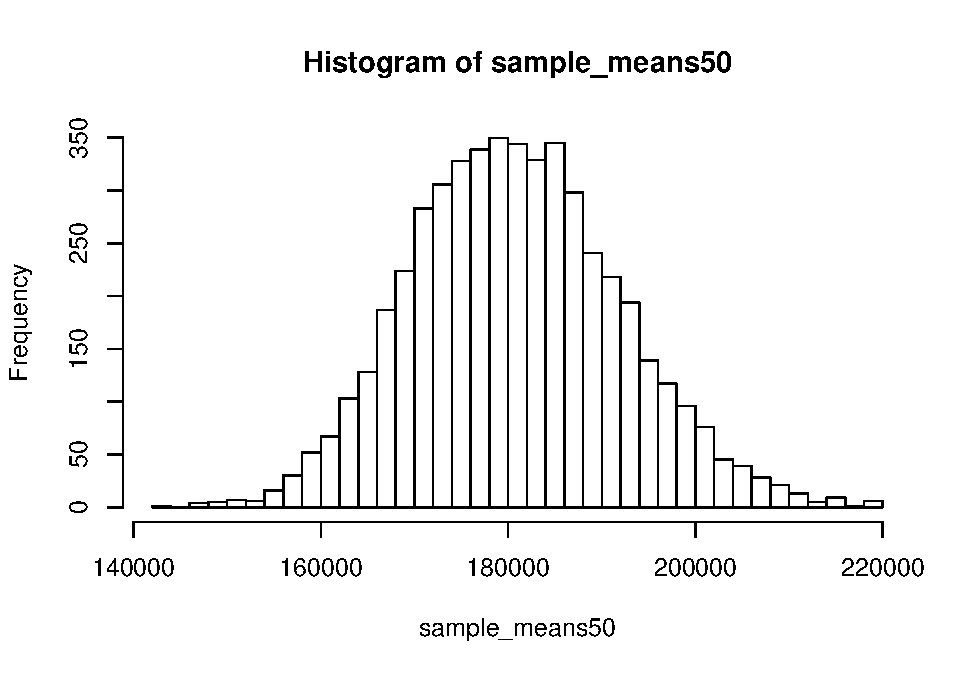
\includegraphics{Lab3A_files/figure-latex/CreateSampleMeans50DistPrice-1.pdf}
\caption{}
\end{figure}

\begin{Shaded}
\begin{Highlighting}[]
\NormalTok{(xsum50 <-}\KeywordTok{summary}\NormalTok{(sample_means50))}
\end{Highlighting}
\end{Shaded}

\begin{verbatim}
##    Min. 1st Qu.  Median    Mean 3rd Qu.    Max. 
##  143300  172900  180400  180800  188000  219500
\end{verbatim}

\textbf{Exercise Answer: The shape of the price sampling distribution is
normal because the median home price of 180.4K is approximately the same
as the mean home price of 180.8K.}

\paragraph{Exercise: Change your sample size from 50 to 150, then
compute the sampling distribution using the same method as above, and
store these means in a new vector called sample\_means150. Describe the
shape of this sampling distribution, and compare it to the sampling
distribution for a sample size of 50. Based on this sampling
distribution, what would you guess to be the mean sale price of homes in
Ames?}\label{exercise-change-your-sample-size-from-50-to-150-then-compute-the-sampling-distribution-using-the-same-method-as-above-and-store-these-means-in-a-new-vector-called-sampleux5fmeans150.-describe-the-shape-of-this-sampling-distribution-and-compare-it-to-the-sampling-distribution-for-a-sample-size-of-50.-based-on-this-sampling-distribution-what-would-you-guess-to-be-the-mean-sale-price-of-homes-in-ames}

\begin{Shaded}
\begin{Highlighting}[]
\NormalTok{sample_means150 <-}\KeywordTok{rep}\NormalTok{(}\OtherTok{NA}\NormalTok{,}\DecValTok{5000}\NormalTok{)}

\NormalTok{for (i in }\DecValTok{1}\NormalTok{:}\DecValTok{5000}\NormalTok{)}
\NormalTok{\{}
     \NormalTok{samp <-}\KeywordTok{sample}\NormalTok{(price, }\DecValTok{150}\NormalTok{)}
     \NormalTok{sample_means150[i] <-}\KeywordTok{mean}\NormalTok{(samp)}
\NormalTok{\}}

\KeywordTok{hist}\NormalTok{(sample_means150, }\DataTypeTok{breaks =} \DecValTok{50}\NormalTok{)}
\end{Highlighting}
\end{Shaded}

\begin{figure}[htbp]
\centering
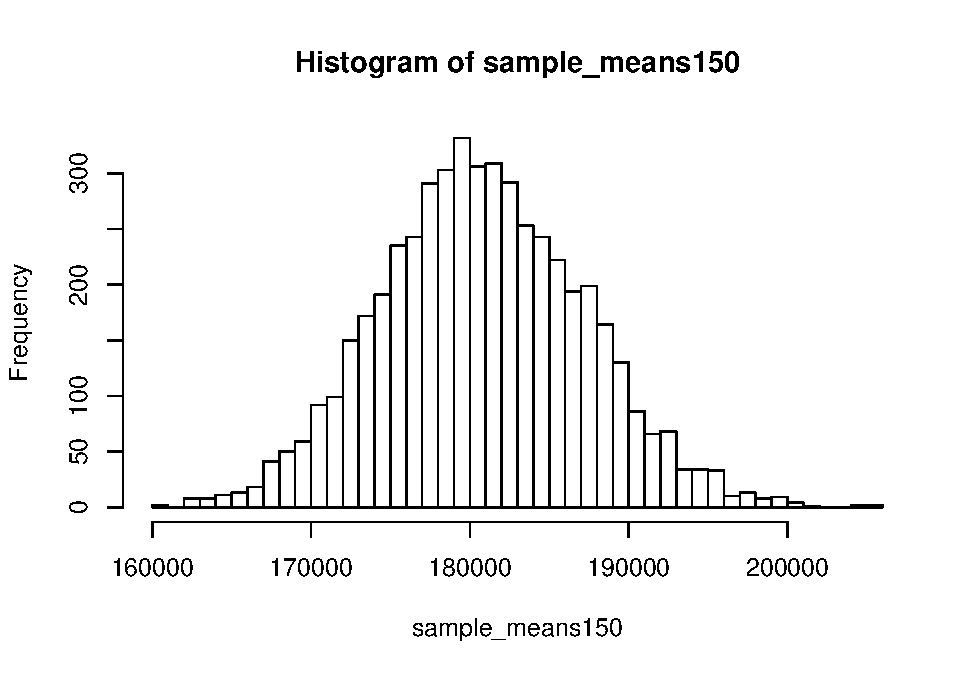
\includegraphics{Lab3A_files/figure-latex/CreateSampleMeans150DistPrice-1.pdf}
\caption{}
\end{figure}

\begin{Shaded}
\begin{Highlighting}[]
\NormalTok{(xsum150 <-}\KeywordTok{summary}\NormalTok{(sample_means150))}
\end{Highlighting}
\end{Shaded}

\begin{verbatim}
##    Min. 1st Qu.  Median    Mean 3rd Qu.    Max. 
##  160300  176500  180600  180800  185100  205400
\end{verbatim}

\begin{Shaded}
\begin{Highlighting}[]
\KeywordTok{par}\NormalTok{(}\DataTypeTok{mfrow =} \KeywordTok{c}\NormalTok{(}\DecValTok{2}\NormalTok{,}\DecValTok{1}\NormalTok{))}
\NormalTok{xlimits50 <-}\KeywordTok{range}\NormalTok{(sample_means50)}
\KeywordTok{hist}\NormalTok{(sample_means50, }\DataTypeTok{breaks =} \DecValTok{50}\NormalTok{, }\DataTypeTok{xlim =} \NormalTok{xlimits50)}
\KeywordTok{text}\NormalTok{(}\DecValTok{210000}\NormalTok{, }\DecValTok{200}\NormalTok{, }\KeywordTok{paste}\NormalTok{(}\StringTok{"Std.Dev ="}\NormalTok{, }\KeywordTok{round}\NormalTok{(}\KeywordTok{sd}\NormalTok{(sample_means50), }\DecValTok{1}\NormalTok{)))}
\KeywordTok{hist}\NormalTok{(sample_means150, }\DataTypeTok{breaks =} \DecValTok{50}\NormalTok{, }\DataTypeTok{xlim =} \NormalTok{xlimits50)}
\KeywordTok{text}\NormalTok{(}\DecValTok{210000}\NormalTok{, }\DecValTok{200}\NormalTok{, }\KeywordTok{paste}\NormalTok{(}\StringTok{"Std.Dev ="}\NormalTok{, }\KeywordTok{round}\NormalTok{(}\KeywordTok{sd}\NormalTok{(sample_means150), }\DecValTok{1}\NormalTok{)))}
\end{Highlighting}
\end{Shaded}

\begin{figure}[htbp]
\centering
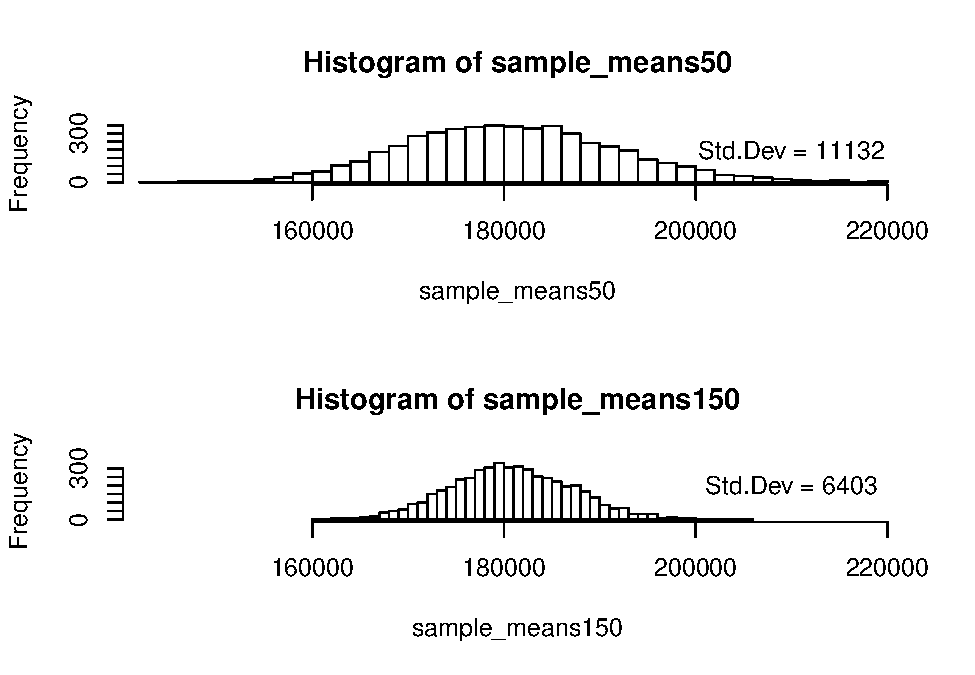
\includegraphics{Lab3A_files/figure-latex/CreateSampleMeans150DistPrice-2.pdf}
\caption{}
\end{figure}

\begin{itemize}
\itemsep1pt\parskip0pt\parsep0pt
\item
  Sample Size 50 Summary:
\end{itemize}

\begin{verbatim}
##    Min. 1st Qu.  Median    Mean 3rd Qu.    Max. 
##  143300  172900  180400  180800  188000  219500
\end{verbatim}

\begin{itemize}
\itemsep1pt\parskip0pt\parsep0pt
\item
  Sample Size 150 Summary:
\end{itemize}

\begin{verbatim}
##    Min. 1st Qu.  Median    Mean 3rd Qu.    Max. 
##  160300  176500  180600  180800  185100  205400
\end{verbatim}

\textbf{Exercise Answer: Both sampling distributions have a near normal
shape. The estimated mean price of homes in Ames is \$184500.}

\paragraph{Question 6: Which of the following is
false?}\label{question-6-which-of-the-following-is-false}

\begin{enumerate}
\def\labelenumi{\Alph{enumi})}
\itemsep1pt\parskip0pt\parsep0pt
\item
  \textbf{The variability of the sampling distribution with the smaller
  sample size (sample\_means50) is smaller than the variability of the
  sampling distribution with the larger sample size (sample\_means150).}
\item
  The means for the two sampling distribtuions are roughly similar.
\item
  Both sampling distributions are symmetric.
\end{enumerate}

\textbf{Question 6 Answer: A is false. Sample sizes of 150 typically
have a smaller sampling distribution spread (45100) than sample sizes of
50 (300500).}

\begin{center}\rule{0.5\linewidth}{\linethickness}\end{center}

\end{document}
